\section{Convergence of empirical risk minimization (ERM)}

\mode<presentation>{
\begin{frame} 
    \begin{center} \huge
        \secname
    \end{center}
\end{frame}
}

\begin{frame}\frametitle{The learning problem}
    \mode<article>{
    \begin{figure}[h]
        \centering
		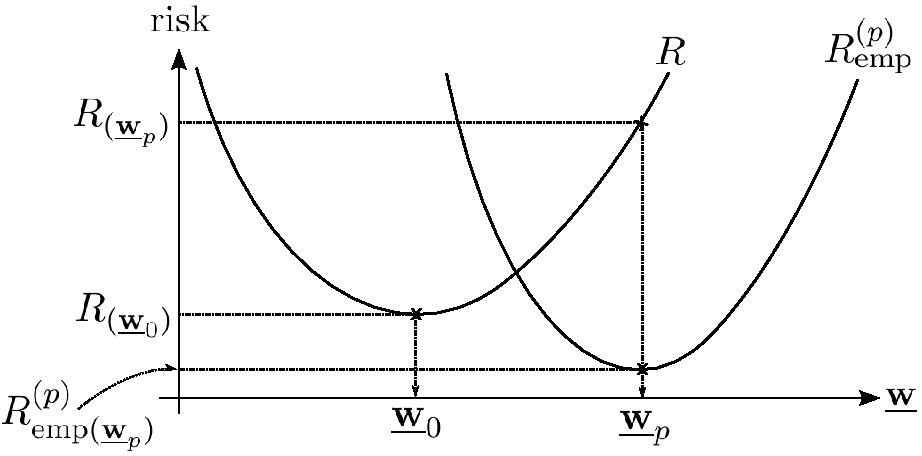
\includegraphics[height=4cm]{img/section2_fig1.pdf}
		\caption{Comparing risk with empirical risk using a finite set with $p$ points.}
	\end{figure}
    }
    \mode<presentation>{
	\placeimage{8}{3}{img/section2_fig1}{width=6cm}
    }
    \underline{Setting}:\\
    
	\begin{itemize}
		\item {\footnotesize samples are drawn \iid~from $P(\vec x, y_T)$\\[1mm]
			 $\quad \leadsto \quad$ $\vec w$ are random variables}
        \item $R_{[\vec w_p]}\,\corresponds\,E^{T}_{[\vec w]}$ \notesonly{:the empirical risk obtained from training the model using a finite set with $p$ points, and}
        \item $R_{[\vec w_{\color{red}0}]}\,\corresponds\,E^{G}_{[\vec w]}$ \\
        \slidesonly{\vspace{5mm}}
        
        Recall that
        \begin{eqnarray} \hspace{5mm} 
			E_{[\vec{w}]}^G 
			&=& \text{probability of misclassification} \\[-1mm]
			&=& \int P_{(y_T, \vec{x})} \,
				e_{(y_T, \vec{x};\vec{w})} \, 
				d \vec{x} \, d y_T \;\;\eqexcl\;\; \min_{\vec w}
		\end{eqnarray}
        
        \notesonly{
        Therefore, $R_{[\vec w_0]}$ represents the risk value obtained from training the model using infinitely many points.
        }
        (Don't treat the ${\color{red}_0}$ as zero data points but rather as ``minimal'' risk)
	\end{itemize}
\end{frame}

% -----------------------------------------------------------------------------
\definecolor{question1}{rgb}{0,0,1}
\definecolor{question2}{rgb}{0,0.5,0}
\begin{frame}\frametitle{When does inductive learning through ERM work?}
	\begin{center} 
	\slidesonly{
		\includegraphics<1-2>[height=4cm]{img/section2_fig1_question1}
		}
		\begin{figure}[h]
			\centering
			\includegraphics<3->[height=4cm]{img/section2_fig1_question2_lessw} 
			\mode<article>{
			\caption{
			Measuring the difference between empirical risk obtained from a finite site of $p$ points with risk obtained using infinitely many points.
			}
			\label{fig:randremp}
			} 
		\end{figure}
	\end{center}
	\only<1>{
	\mode<article>{
	\underline{The key questions of Statistical Learning Theory:}
	}
		\begin{enumerate}
		\slidesonly{
		\vspace{-5mm}
		\item {\footnotesize $p$ samples are drawn \iid~from $P(\vec x, y_T)$\\[1mm]
			 $\quad \leadsto \quad$ $\vec w$ are random variables}
			 }
		\item 
			\vspace{1mm}
			\iitem{$R_{\text{emp}[\vec w_p]}$ 
				should reflect the true optimal risk $R_{[\vec w_0]}$ 
				in the limit $p \to \infty$:}
			\vspace{1mm}
			\begin{equation}
				\lim_{p \rightarrow \infty} P \Big\{ 
						{\color{question1} \big| R_{(\vec{w}_p)}
						- R_{(\vec{w}_0)} \big| }
					\geq \eta \Big\} \;\;=\;\; 0 \,,
					\quad\text{ for all }\quad \eta > 0 \,.
				\label{eq:absdeltaconvergence0}
			\end{equation}
		\end{enumerate}
	} \only<2>{
		\begin{enumerate} \setcounter{enumi}{1}
			\item How strongly does $R_{[\vec{w}_p]}$ differ 
				from $R_{[\vec{w}_0]}$ for  \textbf{finite} samples?
				\vspace{1mm}
				\iitem{For a given confidence $\epsilon$, find $\eta$ such that}
				\vspace{1mm}
				\begin{equation}
					P \Big\{ {\color{question1} 
							\big| R_{[\vec{w}_p]} - R_{[\vec{w}_0]} \big| 
						} \geq \eta \Big\} \;\;<\;\; \epsilon \,.
						\label{eq:convergenceeps}
				\end{equation}
		\end{enumerate}
	} \only<3>{
		\begin{enumerate} \setcounter{enumi}{2}
			\item Do training errors $R_{\text{emp}[\vec w]}$ 
				reflect generalization performance $R_{[\vec w]}$?
				\vspace{1mm}
				\iitem{\footnotesize Avoid overfitting for finite samples,
				i.e.~given confidence $\epsilon$, find $\eta$ such that: 
					%i.e.~$R_{(\vec w)} \approx R_{\mathrm{emp}(\vec w)}$:
				}
				\vspace{1mm}
				\begin{equation}
					P \Big\{ {\color{question2}
							\big| R_{[\vec w]} - R_{\mathrm{emp}[\vec w]} \big|
						} > \eta \Big\} \;\;<\;\; \epsilon \,, 
						\qquad \forall \vec w \in \Lambda \,.
						\label{eq:convergenceepsgeneral}
				\end{equation}
                where $\Lambda$ is the model class (e.g. connectionist neuron)
		\end{enumerate}
	}
\end{frame}

\begin{frame}
\label{sec:convergence_erm}
\frametitle{ Understanding what $P\big\{ 
	{\color{question1}
		\big|R_{[\vec w_p]} - R_{[\vec w_0]}\big| 
	} \geq \eta \big\}$ represents
}

			%And this difference becoming smaller and smaller as we feed more points into the model. That is:
			%\begin{equation}
				%\lim_{p \to \infty} P\bigg\{ 
					%{
						%\Big|R_{[\vec w_p]} - R_{[\vec w_0]}\Big| 
					%}
				%\geq \eta \bigg\}\;\;=\;\; 0 \,, \quad \forall \eta > 0
				%\label{eq:erm_converges_zero}
			%\end{equation}
\mode<presentation>{
	\placeimage{8}{5}{img/section2_fig1_question1}{width=6cm}
}
\begin{figure}
	\mode<article>{ \centering }
	\mode<presentation>{ \raggedright \vspace{-2mm}}
	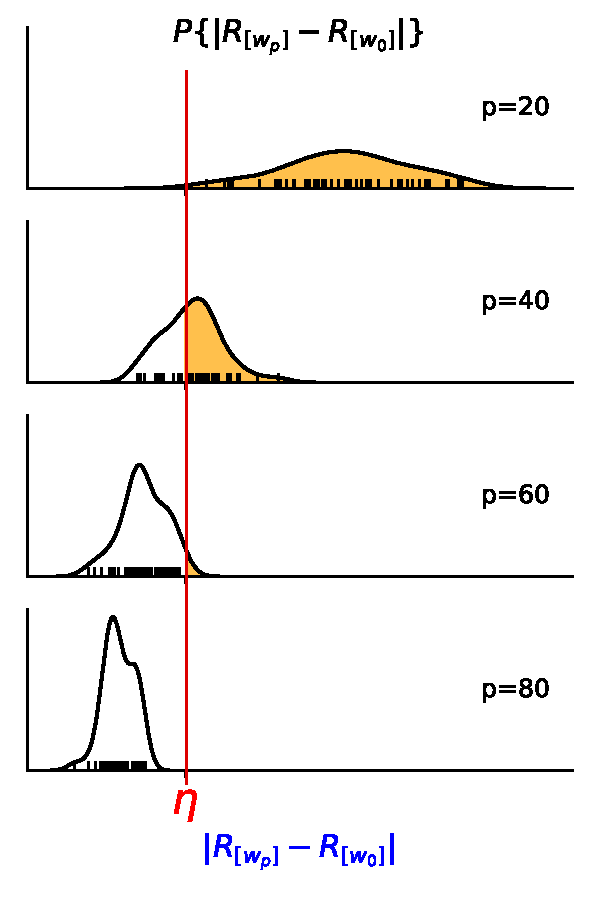
\includegraphics[height=\slidesonly{6.7cm}{\notesonly{8cm}}]{img/PdeltaReta}
	\caption{Distribution of absolute risk differences for larger number of training points $p_{1} < p_{2} < p_{3} < p_{4}$}
	\label{fig:PdeltaReta}
\end{figure}
	
\mode<article>{			
			Understanding \figref{fig:randremp} and
			what\eqref{eq:absdeltaconvergence0} represents:
				
			\begin{itemize}
			\item We expect the model trained on $p$ points to have  some error $R_{\text{emp}}$ that is minimal for some $\vec w_p$ at which the empirical error is $R_{\text{emp}[\vec w_p]}$.
			\item Estimating the generalization performance for the solution $\vec w_p$ on a hold-out set yields a risk value of $R_{[\vec w_p]}$. We expect it to be higher than the optimal risk $R_{[\vec w_0]}$. We therefore measure the absolute difference between both:
			\begin{equation}
			{\color{question1}
			\big| R_{(\vec{w}_p)}
						- R_{(\vec{w}_0)} \big|
						}
			\end{equation}
			\item Training the model with a different set of $p$ points (the size of the training set is kept at $p$) may yield a different minimum for $R_{\text{emp}[\vec w_p]}$ with a corresponding generalization performance $R_{[\vec w_p]}$ and consequently a different absolute difference ${\color{question1}
			\big| R_{(\vec{w}_p)}
						- R_{(\vec{w}_0)} \big|
						}$
			\item Training many models while keeping $p$ fixed will yield many values for the absolute difference ${\color{question1}
			\big| R_{(\vec{w}_p)}
						- R_{(\vec{w}_0)} \big|
						}$
			\item Measuring the absolute difference between every $R_{[\vec w_p]}$ we obtained and $R_{[\vec w_0]}$ will lead to ``difference values'' that follow some distribution $P\big\{ 
					{\color{question1}
						\big|R_{[\vec w_p]} - R_{[\vec w_0]}\big| 
					}
				\geq \eta \big\}$
			\item We measure the probability of the absolute difference exceeding some value $\eta$:
			\begin{equation}
			P\big\{ 
					{\color{question1}
						\big|R_{[\vec w_p]} - R_{[\vec w_0]}\big| 
					}
				\geq \eta \big\}\,, \quad \forall \eta > 0
			\end{equation}
			This is the same asking: How often does training with $p$ points yield a difference in risk above some value.
			\item Now we repeat the training of these models but using a larger value for $p$.\\
			
			What the theory tells you is that as you increase $p$ and keeping $\eta$ fixed:
			\begin{itemize}
				\item The $R_{[\vec w_p]}$ of the models will improve and get smaller.
				\item The absolute differences ${color{question1}\Big|R_{[\vec w_p]} - R_{[\vec w_0]}\Big|}$ will become smaller and smaller,
				\item As depicted by \figref{fig:PdeltaReta}, the distribution of these differences will shift below $\eta$ (i.e. to the left of $\eta$)
				\item Less and less models will score differences $\ge \eta$
				\item Eventually, for some large $p$, the $R_{[\vec w_p]}$ of the models will be so good that the probability of finding a model that has a risk difference of $\eta$ or higher (worse performance) will vanish. And this is what \eqref{eq:risktozero} describes:
			\end{itemize}
			\end{itemize}
			\begin{equation}
				\lim_{p \to \infty} P\bigg\{ 
					{\color{question1}
						\Big|R_{(\vec w_p)} - R_{(\vec w_0)}\Big| 
					}
				\geq \eta \bigg\}\;\;=\;\; 0 \,, \quad \forall \eta > 0
				\label{eq:risktozero}
			\end{equation}
			
			\textbf{But} Our dataset is never going to be infinitely large. Therefore a more realistic formulation for the convergence of ERM would be that it will below some value $\epsilon$:
			\begin{equation}
					P \Big\{ {\color{question1} 
							\big| R_{[\vec{w}_p]} - R_{[\vec{w}_0]} \big| 
						} \geq \eta \Big\} \;\;<\;\; \epsilon \,.
						\label{eq:convergenceeps}
				\end{equation}
				
			Furthermore, recalling what we've learned about the bias-variance tradeoff, the solution that minimizes $R_{\text{emp}}$ might not be a favorable solution. We therefore extend comparison of the curves $R_{\text{emp}}$ with $R$ to include other solutions that do not necessarily minimize the empirical risk $R_{\text{emp}}$ (i.e. training error). This leads to further modifying our formulation of the convergence from \eqref{eq:convergenceeps} to:
				\begin{equation}
					P \Big\{ {\color{question2}
							\big| R_{[\vec w]} - R_{\mathrm{emp}[\vec w]} \big|
						} > \eta \Big\} \;\;<\;\; \epsilon \,, 
						\qquad \forall \vec w \in \Lambda \,.
						\label{eq:convergenceepsgeneral}
				\end{equation}
			
			The key difference between \eqref{eq:convergenceeps} and \eqref{eq:convergenceepsgeneral} is that the latter is no longer restricted to the solutions $\vec w_p$ at which the empirical risk is minimal but may include solutions $\vec w$ that can potentially generalize better.
}
\end{frame}
